\documentclass[conference]{IEEEtran}
\IEEEoverridecommandlockouts
\usepackage{cite}
\usepackage{amsmath,amssymb,amsfonts}
\usepackage{algorithmic}
\usepackage{graphicx}
\usepackage{textcomp}
\usepackage{xcolor}
\usepackage{booktabs}
\usepackage{graphicx}
\usepackage{float}
\usepackage[backend=biber,style=ieee]{biblatex}
\addbibresource{Reference.bib}
% All figures are stored in the fig/ subfolder
\graphicspath{{fig/}}

\def\BibTeX{{\rm B\kern-.05em{\sc i\kern-.025em b}\kern-.08em
    T\kern-.1667em\lower.7ex\hbox{E}\kern-.125emX}}


\begin{document}

\title{Deepfake Detection Using Deep Learning Techniques}

\author{
\IEEEauthorblockN{1\textsuperscript{st} Sameera Kar}
\IEEEauthorblockA{\textit{Center for AI \& ML, ITER} \\
\textit{Siksha `O' Anusandhan University}\\
Bhubaneswar, Odisha, India \\
Email ID : sameerakar05@gmail.com}
\and
\IEEEauthorblockN{2\textsuperscript{nd} Kaibalya Prasad Nayak}
\IEEEauthorblockA{\textit{Center for AI \& ML, ITER} \\
\textit{Siksha `O' Anusandhan University}\\
Bhubaneswar, Odisha, India \\
Email ID: nayakkaibalya021@gmail.com}
\and
\IEEEauthorblockN{3\textsuperscript{rd} Rupali Bisoyi}
\IEEEauthorblockA{\textit{Center for AI \& ML, ITER} \\
\textit{Siksha `O' Anusandhan University}\\
Bhubaneswar, Odisha, India \\
Email ID: rupalibisoyi20@gmail.com }
\and
\IEEEauthorblockN{4\textsuperscript{th} Saswat Kumar Nayak}
\IEEEauthorblockA{\textit{Center for AI \& ML, ITER} \\
\textit{Siksha `O' Anusandhan University}\\
Bhubaneswar, Odisha, India \\
Email ID: saswatofficial2005@gmail.com  }
\and
\IEEEauthorblockN{5\textsuperscript{th} Mr. Abdul Atif Khan}
\IEEEauthorblockA{\textit{Center for AI \& ML, ITER} \\
\textit{Siksha `O' Anusandhan University}\\
Bhubaneswar, Odisha, India}
}

\maketitle

\begin{abstract}
\textbf{The technology of deepfakes has progressed quickly, and with the rapid
progress of deep learning and generative artificial intelligence has made it
possible to generate extremely realistic manipulated images and videos. While
such synthetic media technologies are useful for entertainment and the
generation of media, they also have severe concerns about misinformation,
identity theft, privacy, and cyber security. This paper presents a deepfake
detection framework based on image and video forgery classification with deep
learning methods. The proposed system consists of two parts; an efficient
network model called EfficientNet B0 and a hybrid model of CNN-Transformer for
the classification of real or manipulated facial content. The CelebDF-V2 and FaceForensics++ (FF-C23) datasets are then combined in the preprocessing pipeline followed by face extraction using Multi-task Cascaded Convolutional Networks (MTCNN). To enhance model generalisation, data augmentation, data normalisation and balancing of datasets are carried out. The results of the experimental evaluation show validation accuracy of 99.32\% for EfficientNet B0 and 94.11\% for Hybrid CNN-Transformer. The evaluations of the performance were done by accuracy, precision, recall, F1-score, ROC-AUC analysis, and visualization of confusion matrix. According to the experimental results, the EfficientNet B0 model ismore efficient than the Hybrid CNN-Transformer model in terms of performance,convergence speed, and computational complexity. The proposed framework shows that it is effective of deep learning based architectures for robust and automated deepfake detection.}
\end{abstract}

\begin{IEEEkeywords}
Deepfake Detection, Deep Learning, EfficientNet, CNN-Transformer,
FaceForensics++, CelebDF-V2, Computer Vision, Image Forgery Identification,
Video Forgery, Artificial Intelligence
\end{IEEEkeywords}

%=======================================================
\section{Introduction}
%=======================================================


The technologies of generating multimedia have been transformed rapidly using
Artificial Intelligence and Deep Learning. Among these developments, deepfake
technology has emerged as one of the most powerful and controversial
innovations. Deepfakes are synthetic media generated using deep learning
algorithms that manipulate facial expressions, voice patterns, or identity
information to create highly realistic fake images and videos. Current deepfake
generation methods primarily rely on Generative Adversarial Networks (GANs),
autoencoders, and neural rendering techniques.

Although deepfake technology has beneficial applications in film production,
virtual reality, gaming, digital entertainment, and content creation, its
misuse has become a major global concern. Deepfake media can contribute to
misinformation, fake news propagation, political manipulation, identity theft,
financial fraud, cybercrime, and social engineering attacks. As deepfake
generation techniques continue to evolve, distinguishing manipulated media from
authentic content becomes increasingly difficult.

To address these challenges, automated deepfake detection systems based on deep
learning have gained significant attention in recent years. Convolutional Neural
Networks (CNNs) have proven effective in extracting spatial features from
manipulated facial regions, while transformer-based architectures improve
contextual understanding and capture long-range dependencies.

This research work proposes a deep learning-based framework for deepfake image
and video forgery classification. The framework combines EfficientNet\_B0 and
Hybrid CNN-Transformer architectures for comparative evaluation. During
preprocessing, CelebDF-V2 and FaceForensics++ (FF-C23) datasets are integrated,
followed by facial feature extraction using the MTCNN method for robust facial
representation learning.

The technology used to create deepfakes has advanced significantly and poses
major challenges in verifying the authenticity of digital content. Modern
techniques such as GANs, autoencoders, and neural rendering methods can generate
highly realistic fake facial images and videos that are difficult for humans to
distinguish from authentic media.

The misuse of deepfake technology has raised concerns regarding misinformation,
fake news propagation, political manipulation, identity theft, cybercrime,
financial fraud, and privacy violations. Existing detection systems often
struggle with cross-dataset generalization, computational complexity, and the
detection of high-quality manipulations.

Therefore, there is a strong need for an efficient and robust deepfake detection
framework capable of accurately identifying manipulated media while maintaining
low computational overhead and strong generalization capability across multiple
datasets.


\textit{1) Motivations:} As deepfake generation tools become increasingly
accessible, synthetic media creation has become easier and more widespread. The
rapid spread of manipulated media through social media platforms and digital
communication systems has increased the risks associated with misinformation and
identity impersonation.

The traditional forensic techniques are often not enough to identify advanced
deepfake manipulations. The idea of automated deep learning is fostered by this motivation.
Systems for learning that detect minute discrepancies in manipulated
facial content.

In addition, the advances in CNN and transformer based architectures offer
opportunities for developing more accurate and computationally efficient deepfake
detection models.

\textit{2) Objectives:} The main goal of this research project is to
Build an automated deep fake detector with deep learning algorithms.
that are hard to detect for identification of manipulated facial images and videos.
through visual inspection.

The framework proposed uses EfficientNet\_B0 and Hybrid CNN-Transformer.
architectures for deepfake classification and utilizes MTCNN for facial feature
The extraction to enhance facial feature representation.

This research also focuses on integrating CelebDF-V2 and FaceForensics++ datasets
For mass training and assessment. Advanced processing of data and preprocessing.
Several augmentation techniques are used to enhance the robustness of the model and
generalization capability.

Moreover, the suggested models are assessed with several performance criteria
You can include accuracy, precision, recall, F1-score, ROC-AUC score and confusion.
matrix analysis. A comparative analysis is done between EfficientNet\_B0 and
Subsequently, hybrid CNN-Transformer networks were introduced to determine which model is the best one to use.
deepfake detection.
\textit{3) Scope:} We are interested in this research area targeting deepfakes image and video detection.
using deep learning techniques. The proposed framework is aimed at the identification of
Advanced synthetic media generation that creates facial content that is manipulated.
technologies.

The work includes deepfake image and video classification, facial feature
The comparative analysis of EfficientNet\_B0 with MTCNN is provided in the extraction process.The comparative analysis between EfficientNet\_B0 and MTCNN is provided in extraction process.
Hybrid CNN-Transformer models based on classification accuracy and
computational efficiency.

The proposed framework is trained and tested with benchmark datasets
Such as CelebDF-V2 and FaceForensics++. The implementation is carried out in a
GPU-based deep learning environment that enables efficient training of models.
large-scale experimentation.

The current study focuses on the detection of deepfakes of faces only, and does not consider
It can be audio-only deep fake detection or multimodal forensic analysis.

\textit{4) Significance:}As the use of synthetic media continues to grow,
technologies, deepfake detection has emerged as an important research area. The
proposed framework helps to mitigate risks of manipulated
digital content and enhancing the systems for authenticating media.

The impact of this research is on the improvement of cybersecurity and digital media.
Automated deepfake detection methods for verification. The framework
Provides information to combat misinformation, propagation of fake media and manipulation of digital content.
content which is available on the internet. It also enhances automated forensics analysis.
Incorporating deep learning-based architectures in order to detect manipulated facial images.
and videos.

Furthermore, the proposed system is efficient in terms of computation and accurate.
An enhanced generalization deepfake detection framework. The study
further highlights the need for ongoing research and development of
Artificial Intelligence (AI) Media Forensics and Deepfake Detection.
technologies.


%=======================================================
\section{Review of Literature}
%=======================================================

Deepfake detection has emerged as an important research area due to the rapid advancement of generative artificial intelligence and synthetic media technologies. Several deep learning-based approaches have been proposed to identify manipulated images, videos, and audio content.

Pravallika and Tejaswini \cite{b1} proposed a deep learning-based framework for detecting manipulated images and videos using advanced convolutional architectures. Their study emphasized automated forensic analysis for maintaining digital media authenticity.

Srinivasan et al. \cite{b2} developed a Deepfake Detection Model (DDM) integrating GANs, Autoencoders, and CNNs for real-time facial forgery detection. Their system achieved promising results on benchmark datasets.

Ekatpure et al. \cite{b3} introduced a hybrid CNN-LSTM framework capable of detecting deepfake images, videos, and audio content by learning both spatial and temporal manipulation features.

Deshpande et al. \cite{b4} presented a CNN-based deepfake detection system that achieved high classification accuracy through optimized preprocessing and feature extraction techniques.

Soppari et al. \cite{b5} conducted a comprehensive survey of deepfake detection algorithms and highlighted the effectiveness of CNN and EfficientNet-based architectures in identifying subtle facial inconsistencies.

Abhineswari et al. \cite{b6} performed a comparative study using transfer learning models such as MobileNetV2 and ResNet50 on FaceForensics++, demonstrating the effectiveness of pretrained neural networks.

Bagherzadeh and Rastgoo \cite{b7} proposed a hybrid deep convolutional neural network architecture for deepfake image detection, improving robustness across large-scale datasets.

Jheelan and Pudaruth \cite{b8} evaluated several pretrained deep learning models including MobileNet and InceptionV3 and achieved high detection accuracy on GAN-generated deepfakes.

Patel et al. \cite{b9} reviewed recent deepfake detection approaches including CNNs, transformers, LSTMs, and multimodal architectures while identifying challenges related to dataset bias and model generalization.

Kosarkar and Sakarkar \cite{b10} proposed a VARMA-LSTM-GRU architecture for spatio-temporal analysis of manipulated facial content, demonstrating improved detection performance on complex deepfake datasets.

Research in the last few years has emphasized the issue of cross-dataset robustness. CNN architectures with robust performance on other data sets have been shown to generalize well and possess better robustness against sophisticated attacks \cite{b11}.

Multi-modal learning involving multiple sources of information such as visual, temporal, and auditory signals has proven to be effective in deepfake detection with enhanced accuracy \cite{b12,b13}.

With the increasing use of AI to create media, the need for more sophisticated and scalable deepfake detection systems for cybersecurity, journalism, and digital forensics applications has increased \cite{b14}.

There has been recent interest in applying Explainable Artificial Intelligence (XAI) to CNN models to enhance their interpretability and improve their reliability \cite{b15}.

Modern deep learning frameworks that exploit spatial-temporal features have been demonstrated to detect deepfake videos with higher accuracy \cite{b16,b18}.

AI image forensic frameworks that can detect abnormalities due to manipulation using visual inconsistencies in texture have shown excellent accuracy rates in detecting manipulated facial images \cite{b17,b22}.

Combining the benefits of CNN architecture with attention mechanisms has yielded hybrid architectures that exhibit better classification accuracy than standard CNN architectures \cite{b19,b26}.

Research comparing deep learning approaches to traditional machine learning methods shows the superiority of neural networks in detecting deepfakes accurately \cite{b20}.

Interpretable model design, especially regarding deepfake video detection, is an area worth exploring further in order to improve trust in artificial intelligence frameworks \cite{b21}.

Temporal deep learning methods that exploit visual and non-visual cues from deepfake videos to detect manipulation show promising results \cite{b23,b24,b25}.

However, while existing approaches offer high detection accuracy, issues such as cross-dataset generalization, computational efficiency, adversarial attacks, and the ability to detect highly realistic fake videos remain challenging problems.


The main limitation in the current deepfake detection literature is the ubiquitous use
of intra-dataset evaluation protocols, which greatly hinders cross-dataset generalisation.
Most existing models are trained, validated, and tested within a single isolated repository
such as FaceForensics++ or CelebDF-V2. Consequently, these networks inadvertently
overfit to the unique blending artefacts, specific illumination profiles, and proprietary
compression algorithms inherent to a particular dataset. However, their classification accuracy drops drastically when challenged with unseen datasets or real-world multimedia
content. This vulnerability exposes a fundamental flaw in domain adaptability and indicates the absence of reliable invariant feature extraction techniques capable of recognising
the inherent statistical anomalies shared by all synthetic media rather than the digital
signatures of a specific dataset.

In addition, while CNNs can effectively learn localised spatial features and highfrequency edge inconsistencies within facial patches, their local receptive fields are inherently incapable of modelling long-range global dependencies between different facialregions. This limitation is further exacerbated by the fact that few studies integrate a
comprehensive set of diverse deepfake generation techniques such as FaceSwap, Face2Face,
NeuralTextures, and FaceShifter into a unified training and evaluation pipeline. Existing
frameworks, which are limited to specific isolated forgery modalities, remain vulnerable
to hybrid or emerging synthetic generation methods, thereby highlighting a significant
gap in the development of universally robust forensic systems.

%=======================================================
\section{Materials and Methods}
%=======================================================


\subsection{System Architecture}

The proposed deepfake detection framework follows a sequential processing
pipeline consisting of dataset collection, preprocessing, feature extraction,
model training, and classification.

The proposed system begins with collecting benchmark datasets including CelebDF-V2
and FaceForensics++ (FF-C23). The collected video samples are converted into image
frames using frame extraction techniques. Facial regions are then detected and
extracted using Multi-task Cascaded Convolutional Networks (MTCNN).

The extracted facial images undergo preprocessing and data augmentation operations
such as resizing, normalization, rotation, flipping, and brightness adjustment to
improve model generalization. After preprocessing, deep learning models perform
feature extraction and classification to distinguish between real and fake facial
content.

Finally, the performance of the proposed framework is evaluated using multiple
evaluation metrics including accuracy, precision, recall, F1-score, ROC-AUC score,
and confusion matrix analysis.

The proposed framework integrates EfficientNet\_B0 and Hybrid CNN-Transformer
architectures for comparative deepfake classification.

\begin{figure*}[!htbp]
    \centering
    \includegraphics[width=1.8\columnwidth]{3.5.png}
    \caption{Architecture of EfficientNetB012}
    \label{fig:Architecture of EfficientNetB 012}
\end{figure*}

\begin{figure*}[!htbp]
    \centering
    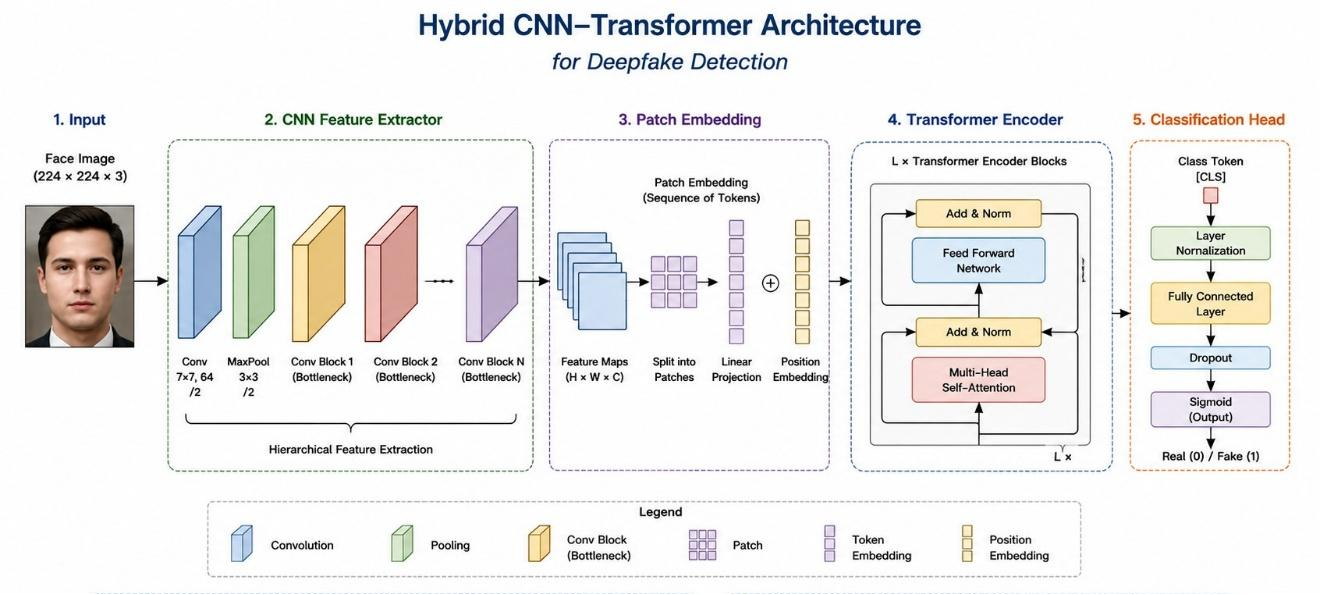
\includegraphics[width=1.8\columnwidth]{3.6.png}
    \caption{Architecture of Hybrid CNN Transformer model}
    \label{fig:Architecture of Hybrid CNN Transformer model}
\end{figure*}

\subsection{Methodology}

The proposed methodology begins with collecting deepfake datasets from CelebDF-V2
and FaceForensics++ repositories. Videos are converted into image frames using
frame extraction techniques.

The extracted frames are processed using Multi-task Cascaded Convolutional
Networks (MTCNN) for facial region detection and extraction. The facial images are
resized and normalized before being provided as input to the deep learning models.

To improve model generalization and reduce overfitting, data augmentation
techniques such as horizontal flipping, rotation, brightness adjustment, random
cropping, and noise injection are applied.

The proposed framework implements two deep learning architectures for deepfake
classification. EfficientNet\_B0 is a lightweight CNN architecture that uses
compound scaling to balance network depth, width, and image resolution. The model
efficiently extracts spatial manipulation features from facial images while
maintaining low computational complexity and fast convergence.

The second model is a Hybrid CNN-Transformer architecture that combines CNN layers
with transformer-based attention mechanisms. CNN layers extract low-level spatial
features from facial regions, while transformer encoder layers capture long-range
contextual dependencies and inconsistencies present in deepfake media.

\begin{figure}[!htbp]
    \centering
    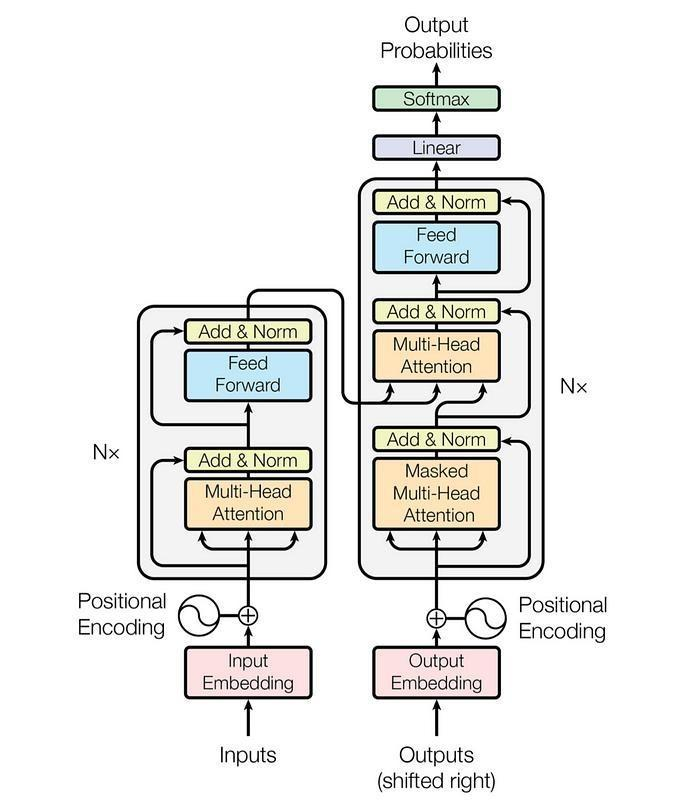
\includegraphics[width=0.7\columnwidth]{3.4.png}
    \caption{System Architecture of the Proposed Deepfake Detection Framework}
    \label{fig:system_architecture}
\end{figure}

\newpage
\subsection{Tools, Technologies and Frameworks Used}

The proposed framework was implemented using Python-based deep learning libraries
along with GPU acceleration support for efficient model training and evaluation.

The tools and technologies used in this research are listed below:

\begin{table}[htbp]
\caption{Tools and Technologies Used}
\begin{center}
\begin{tabular}{|l|l|}
\hline
\textbf{Tool / Framework} & \textbf{Purpose} \\
\hline
Python               & Programming Language \\
TensorFlow / PyTorch & Deep Learning Framework \\
OpenCV               & Image and Video Processing \\
MTCNN                & Face Detection and Extraction \\
NumPy                & Numerical Computation \\
Matplotlib           & Visualization and Graph Plotting \\
Kaggle Notebook      & GPU-based Training Environment \\
NVIDIA Tesla T4      & GPU Acceleration \\
\hline
\end{tabular}
\label{tab2}
\end{center}
\end{table}
Python was used as the primary programming language for implementing the proposed deepfake detection framework due to its simplicity, flexibility, and extensive support for machine learning and computer vision libraries. TensorFlow and PyTorch deep learning frameworks were utilized for designing, training, and evaluating the EfficientNet B0 and Hybrid CNN-Transformer models. These frameworks provide GPU acceleration support, pretrained model architectures, automatic differentiation, and efficient tensor computation for large-scale deep learning applications. OpenCV was used for image and video preprocessing operations including frame extraction, image resizing, normalization, facialregion manipulation, and video handling. OpenCV provides optimized computer vision
utilities that improve preprocessing efficiency. MTCNN was employed for robust facial region detection and alignment. The cascaded architecture of MTCNN enables accurate face localization even under varying illumination conditions, facial orientations, and
image quality degradations. NumPy was used for numerical computation, matrix operations, tensor manipulation, and efficient handling of multidimensional arrays during preprocessing and model training. Matplotlib was utilized for visualization and graphical
representation of training accuracy, loss curves, confusion matrices, ROC curves, and comparative performance analysis of the proposed models. The experiments were conducted using Kaggle Notebook with NVIDIA Tesla T4 GPU 14 acceleration support. GPU-based computation significantly reduced model training time and enabled efficient
large-scale deep learning experimentation.


%=======================================================
\section{Results and Discussion}
%=======================================================

\subsection{Dataset Description}

The proposed deepfake detector system uses two benchmark public datasets for its performance evaluation: CelebDF-V2 and FaceForensics++. CelebDF-V2 dataset comprises high-quality videos consisting of synthetically generated faces similar to real ones without any visual artifacts, thus enabling to test deepfake detectors on real-world data. The data set includes real and fake videos of celebrities for classification. Another widely known facial forgery dataset for evaluation purposes is FaceForensics++ (FF-C23), which contains videos created by manipulating real videos through the application of several face editing methods like Deep Fakes, FaceSwap, Face2Face, and NeuralTextures. The main idea of this dataset is the evaluation of deep learning-based forgery detection methods via applying various manipulations and different compression levels. For this research project, both data sets will be used at first with face extraction and subsequent detection of face region using MTCNN approach. The detected faces will be normalized and combined into a unified dataset for the further use in training, validation and testing process.

In the experiment, two major data sources were utilized; CelebDF-V2 images data set, and FaceForensics++C23 video data set. The CelebDF-V2 component of the data source includes images which are categorized into train, validation, and test splits with real and fake labels. On the other hand, the FaceForensics++C23 video data set has video files in .mp4 formats. Original video files are considered as real while those in manipulated videos in Deepfakes, Face2Face, FaceSwap, Neuraltextures, FaceShifter, and DeepFakeDetection are considered fake. It is a technically sound approach of combining the two data sources because CelebDF-V2 includes image data with identities while FaceForensics++ includes frames from manipulations. 
Following the data pre-processing and concatenation procedures, the notebook reveals that the data counts in the concatenated dataset are: Train real= 40933 images, Train fake= 41254 images, Val real= 5718 images, Val fake= 5762 images, Test real= 5742 images, and Test fake= 5805 images. In the course of training the model, the notebook uses the concatenated training directory to create a dataframe and performs a stratified train test split with test size of 0.2 and gets 65749 images for training and 16438 images for validation. The test directory consists of 11547 images. Given a batch size of 64, this results in 1028 batches of training images, 257 batches of validation images, and 181 batches of test images.

The dataset distribution after preprocessing is summarized below:

\begin{table}[htbp]
\caption{Dataset Distribution After Preprocessing}
\begin{center}
\begin{tabular}{|l|c|c|c|}
\hline
\textbf{Dataset Split} & \textbf{Real Images} & \textbf{Fake Images} & \textbf{Total Images} \\
\hline
Training Set   & 40,933 & 41,254 & 82,187 \\
Validation Set & 5,718  & 5,762  & 11,480 \\
Test Set       & 5,742  & 5,805  & 11,547 \\
\hline
\end{tabular}
\label{tab1}
\end{center}
\end{table}

\subsection{Performance Metrics / Evaluation Criteria}

The proposed framework was evaluated using multiple performance metrics to analyze
classification effectiveness.

\textit{1) Accuracy:} Accuracy measures the overall percentage of correctly
classified samples.
\begin{equation}
Accuracy = \frac{TP + TN}{TP + TN + FP + FN}
\end{equation}

\textit{2) Precision:} Precision measures the proportion of correctly predicted
fake samples among all predicted fake samples.
\begin{equation}
Precision = \frac{TP}{TP + FP}
\end{equation}

\textit{3) Recall:} Recall measures the ability of the model to correctly identify
fake samples.
\begin{equation}
Recall = \frac{TP}{TP + FN}
\end{equation}

\textit{4) F1-Score:} F1-score provides a balanced evaluation between precision
and recall.
\begin{equation}
F1 = \frac{2 \times Precision \times Recall}{Precision + Recall}
\end{equation}

\textit{5) ROC-AUC Score:} ROC-AUC evaluates the model's capability to distinguish
between real and fake samples across multiple classification thresholds.

\textit{6) Confusion Matrix:} The confusion matrix provides detailed visualization
of true positives, true negatives, false positives, and false negatives for
deepfake classification performance analysis.

The proposed deepfake detection pipeline was evaluated on the combined Celeb-DF v2
image dataset and FaceForensics++ C23 video-frame dataset after face extraction and
dataset merging. The final training subset contained 82,187 images, which was
further divided into 65,749 training images and 16,438 validation images. A
separate test directory containing 11,547 images was also prepared during
preprocessing. All images were resized to $224 \times 224$, normalized using
ImageNet statistics, and trained with a batch size of 64 for 20 epochs. The
training procedure used AdamW optimization, weight decay of $10^{-4}$, label
smoothing of 0.1, cosine annealing learning-rate scheduling, automatic mixed
precision, gradient clipping, and a warm-up phase in which the pretrained backbone
was initially frozen.

EfficientNet\_B0 demonstrated fast and stable convergence, as shown in
Fig.~\ref{fig:eff_acc} and Fig.~\ref{fig:eff_loss}. During the first four epochs,
the model improved gradually from 65.72\% training accuracy and 67.66\% validation
accuracy to 70.19\% and 71.86\%, respectively. A sharp improvement occurred after
backbone unfreezing, where the validation accuracy increased to 88.45\% at epoch 5
and 95.30\% at epoch 6. The final validation accuracy reached 99.32\%, with a
validation loss of 0.2126. The close alignment between training and validation
accuracy indicates strong generalization without evident overfitting.

% ---- Figure 1 ------------------------------------------------
\begin{figure}[htbp]
  \centerline{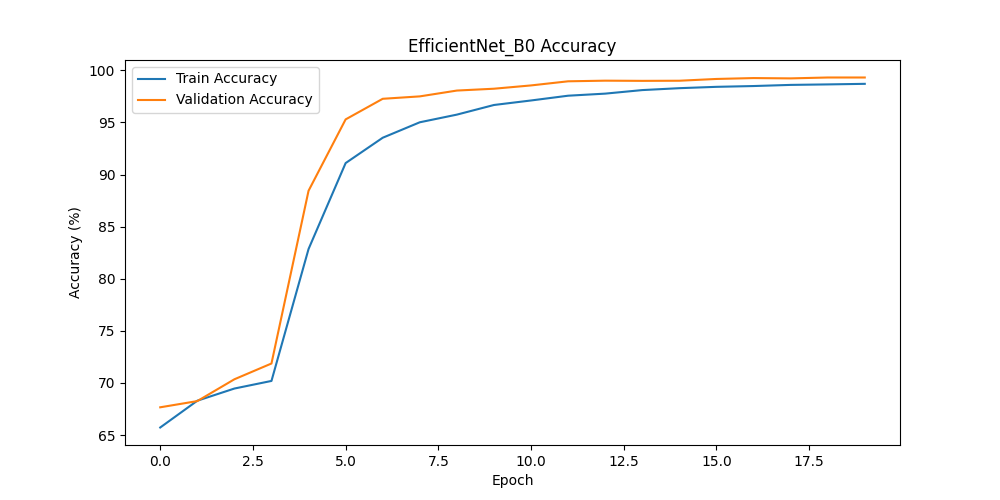
\includegraphics[width=\columnwidth]{efficientnet_accuracy.png}}
  \caption{Training and validation accuracy of EfficientNet\_B0.}
  \label{fig:eff_acc}
\end{figure}

% ---- Figure 2 ------------------------------------------------
\begin{figure}[htbp]
  \centerline{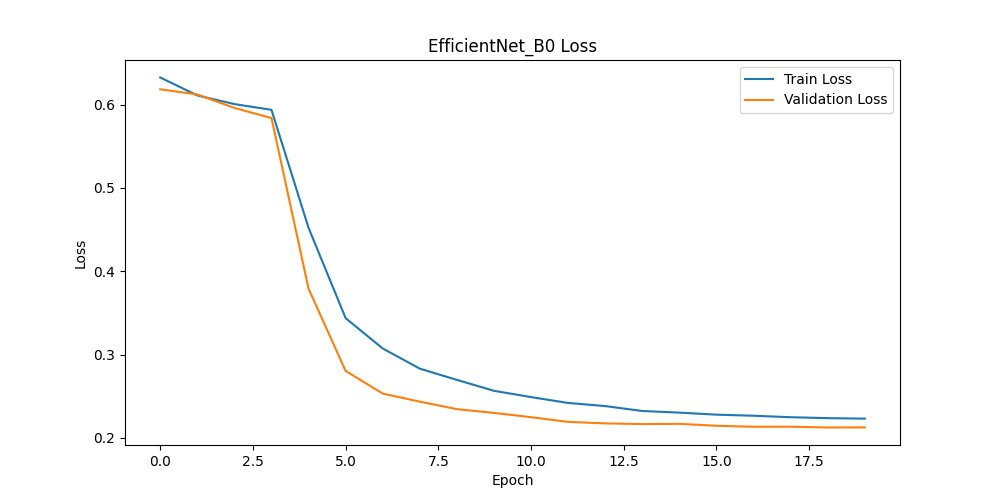
\includegraphics[width=\columnwidth]{efficientnet_loss.png}}
  \caption{Training and validation loss of EfficientNet\_B0.}
  \label{fig:eff_loss}
\end{figure}

The CNN-Transformer model also showed consistent convergence, although at a slower
rate than EfficientNet\_B0. As shown in Fig.~\ref{fig:cnn_acc}, the validation accuracy rose from 67.90\% in epoch 1 to 94.11\% in epoch 20. The associated loss function plot presented in Fig.~\ref{fig:cnn_loss} fell from 0.6107 to 0.2933, indicating continued optimization without significant fluctuations. In the hybrid model employed, EfficientNet convolution layers were leveraged for extracting facial features, which were then processed by the transformer encoder containing 49 spatial tokens and 256 dimensions per token. This helped the network to extract relationships between facial regions at different locations,
rather than using just local convolutional features.

% ---- Figure 3 ------------------------------------------------
\begin{figure}[htbp]
  \centerline{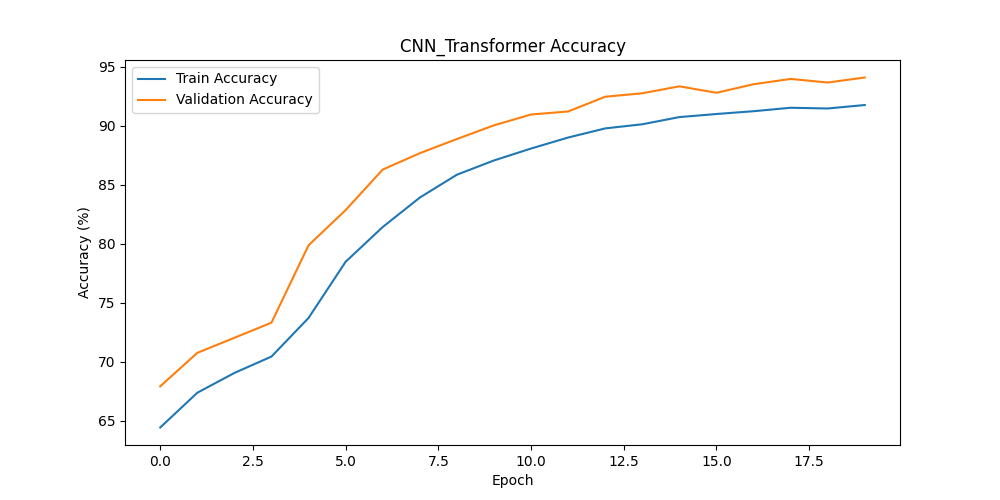
\includegraphics[width=\columnwidth]{cnn_transformer_accuracy.png}}
  \caption{Training and validation accuracy of the CNN-Transformer model.}
  \label{fig:cnn_acc}
\end{figure}

% ---- Figure 4 ------------------------------------------------
\begin{figure}[htbp]
  \centerline{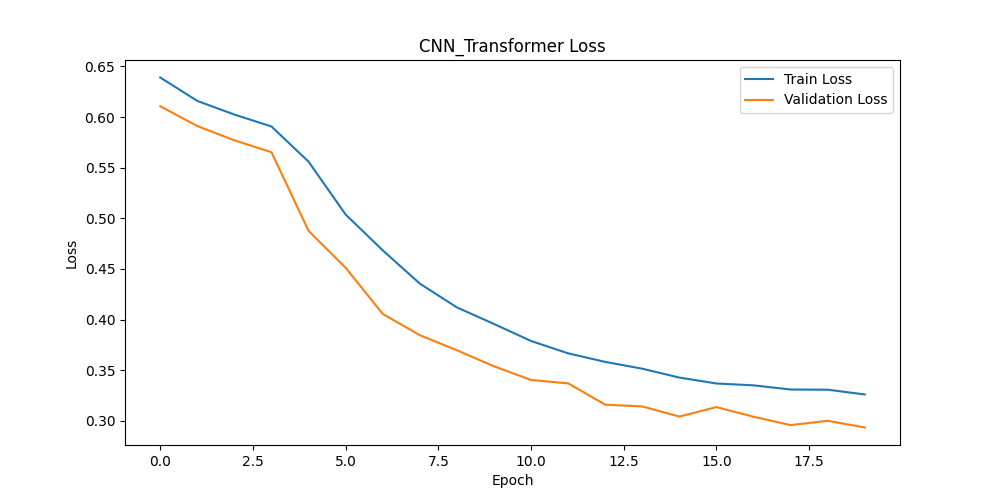
\includegraphics[width=\columnwidth]{cnn_transformer_loss.png}}
  \caption{Training and validation loss of the CNN-Transformer model.}
  \label{fig:cnn_loss}
\end{figure}

EfficientNet\_B0 converged faster and achieved the highest validation accuracy, whereas the CNN-Transformer improved more gradually throughout training. The difference is mainly due to the additional transformer parameters and the requirement to learn token-level spatial relationships after convolutional feature extraction. Although the transformer-based model did not exceed EfficientNet\_B0 in this experiment, its smoother convergence behavior suggests improved structural representation learning and enhanced sensitivity to global facial dependencies. In contrast, EfficientNet\_B0 benefited from a compact and highly optimized
convolutional backbone, making it computationally more efficient with lower GPU
utilization and faster convergence.

The confusion matrix of EfficientNet\_B0 in Fig.~\ref{fig:conf_eff} shows strong
class separation. With fake images encoded as class 0 and real images encoded as
class 1, the model produced 8,187 true negatives and 8,139 true positives, with
only 64 false positives and 48 false negatives. This indicates balanced recognition
of both real and fake samples. The model achieved 99.32\% accuracy, 99.22\%
precision, 99.41\% recall, and an F1-score of 99.32\%.

% ---- Figure 5 ------------------------------------------------
\begin{figure}[htbp]
  \centerline{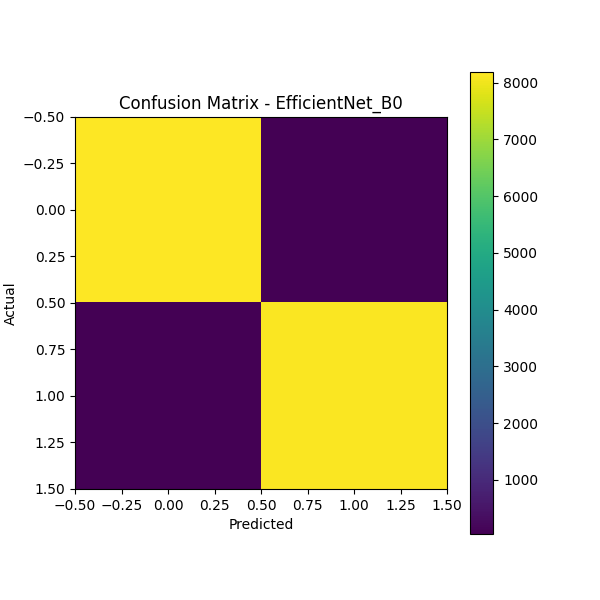
\includegraphics[width=\columnwidth]{confusion_efficientnet.png}}
  \caption{Confusion matrix of EfficientNet\_B0 on the validation split.}
  \label{fig:conf_eff}
\end{figure}

The CNN-Transformer confusion matrix in Fig.~\ref{fig:conf_cnn} shows 7,584 true
negatives and 7,885 true positives, with 667 false positives and 302 false
negatives. The model achieved 94.11\% accuracy, 92.20\% precision, 96.31\% recall,
and an F1-score of 94.21\%. The higher recall indicates that the transformer-based
model was effective at identifying real samples, but the larger number of false
positives shows that it more frequently classified fake samples as real. This
behavior suggests that the hybrid model learned broader spatial dependencies but
required stronger discrimination for subtle localized artifacts that are efficiently
captured by convolutional filters.

% ---- Figure 6 ------------------------------------------------
\begin{figure}[htbp]
  \centerline{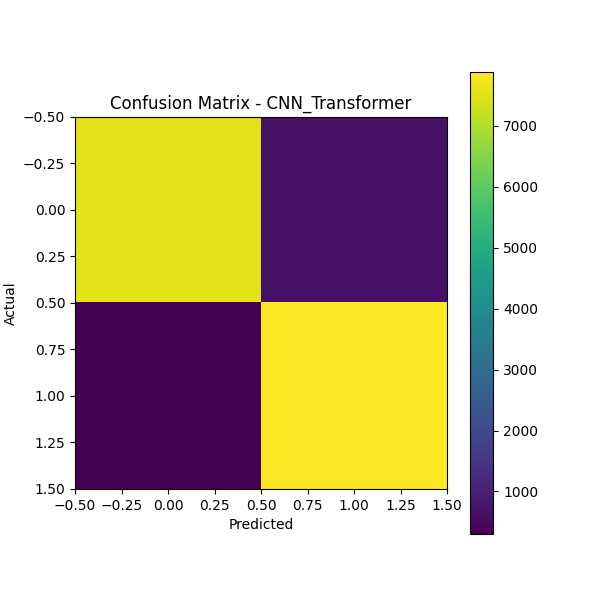
\includegraphics[width=\columnwidth]{confusion_cnn_transformer.png}}
  \caption{Confusion matrix of the CNN-Transformer model on the validation split.}
  \label{fig:conf_cnn}
\end{figure}

\begin{table}[htbp]
\caption{Performance Comparison of Proposed Models}
\begin{center}
\begin{tabular}{|l|c|c|c|c|}
\hline
\textbf{Model} & \textbf{Accuracy} & \textbf{Precision} & \textbf{Recall} & \textbf{F1-score} \\
\hline
EfficientNet\_B0 & 99.32\% & 99.22\% & 99.41\% & 99.32\% \\
CNN-Transformer  & 94.11\% & 92.20\% & 96.31\% & 94.21\% \\
\hline
\end{tabular}
\label{tab3}
\end{center}
\end{table}

As can be seen from Fig.~\ref{fig:final_cmp} and Table~\ref{tab3}, the last
comparison shows that the EfficientNet\_B0 model was the most effective in
performance and computation. The architecture being lightweight, the pretrained
hierarchy of features, and quick convergence of this model makes it fit to be used
in deepfake recognition systems in real-life situations when speed and GPU
computation are considered. The CNN-Transformer consumed relatively more computing
power and converged relatively slower than EfficientNet\_B0, but the key
advantage of using it is the self-attention mechanism over the spatial feature
tokens.

% ---- Figure 7 ------------------------------------------------
\begin{figure}[htbp]
  \centerline{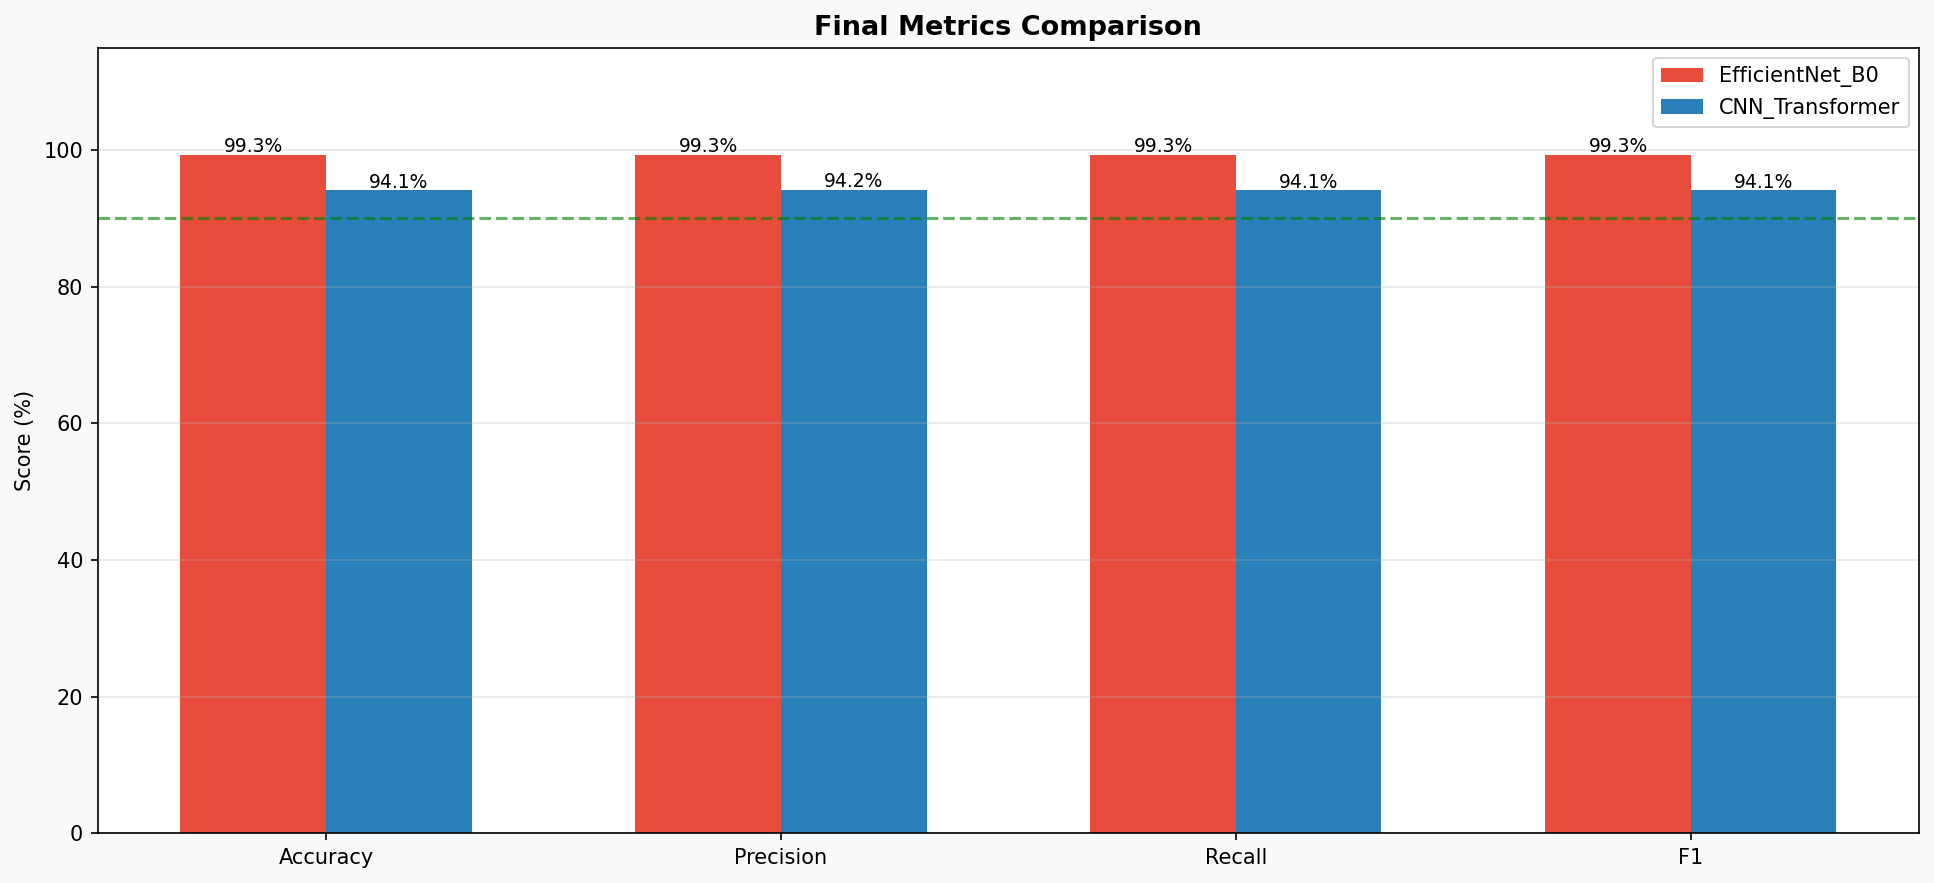
\includegraphics[width=\columnwidth]{final_metrics_comparison.png}}
  \caption{Final metric comparison of EfficientNet\_B0 and CNN-Transformer.}
  \label{fig:final_cmp}
\end{figure}

Overall, the experimental evaluation demonstrates that both architectures
effectively learned discriminative deepfake representations from facial regions.
EfficientNet\_B0 achieved superior classification accuracy and computational
efficiency, whereas the CNN-Transformer exhibited stronger global spatial
dependency modeling. The obtained results confirm the effectiveness of deep
learning-based facial feature analysis for robust deepfake detection.
\section{Conclusion}

In this research a convolutional neural networks (CNN) based model is proposed.
We pretrained the models on the benchmark CelebDFV2 and FaceForensics++ (FF-C23) for deepfake detection tasks. The proposed framework used MTCNN for face extraction and compared the performance of two deep learning architectures (EfficientNet B0 and a Hybrid CNN-Transformer) for the task of real face/fake face classification of facial content.

Experimental results showed the ability of both these models to detect the presence of Deepfakes, with EfficientNet B0 having the best performance with a validation accuracy of 99.32\%, precision of 99.22\%, recall of 99.41\%, and F1-score of 99.32\%. The Hybrid CNN-Transformer model produced 94.11\% accuracy of the validation set and showed a good ability to capture global spatial dependencies via its attention mechanism.

The results suggest that EfficientNet B0 is better for the classification task, has quicker convergence and lower computational complexity, which makes it more useful for practical deepfake detection applications. The study validates the efficacy of using the facial feature analysis due to the use of deep learning algorithm for detecting manipulated images and video frames. This improvement has also strengthened by using sophisticated preprocessing process, data augmentation, and face extraction, which enhanced the generalization and accuracy of the face detection.

For future research, various extensions can be considered, including the extension to multimodal information (such as audio or text), the enhancement of adversarial attack resistance in deepfake detection, and the study of Explainable Artificial Intelligence (XAI) to boost the interpretability and reliability of deepfake detection systems in realistic settings.



\section{Future Scope}

The algorithms used for generating deepfakes are still evolving rapidly, and it is a key research area to create more powerful algorithms for detecting faux faces. A possible line of research is to make better use of cross-dataset generalization, where detection models are able to perform well when trained on an unseen set of input media. This can be achieved by using novel domain adaptation and self-supervised learning methods.

In the future, multimodal deepfake detection (combining visual and audio information and text) will be investigated in addition to the aforementioned. This can enable more thorough analysis and more accurate detection of the more complex deepfake material. Beyond that, transformer structures and vision-language models may be considered to be able to encode the richer contextual pattern in manipulated media.

An emerging strategy is the use of Explainable Artificial Intelligence (XAI) methods to enhance the transparency and interpretability of the models. Knowledgeable detection systems can provide explanation to the reasons underlying classification decisions and boost the confidence in an automatic forensic tool.

In addition, future investigation of adversarially robust deepfake detectors---those resistant to attacks that are created to fool the detection systems---is possible. Another critical aspect of deepfakes is the need for real-time deployment of detection systems across social media platforms, cybersecurity systems, and digital forensic tools. These developments will help increase the reliability and scalability of measures to fight against misinformation and make electronic media trustworthy.

%=======================================================



\nocite{*}
\printbibliography

\end{document}
